%%%%%%%%%%%%%%%%%%%%%%%%%%%%%%%%%%%%%%%%%%%%%%%%%%%%%
%   Chapter 1: Basic concepts in of Machine leaning %
%%%%%%%%%%%%%%%%%%%%%%%%%%%%%%%%%%%%%%%%%%%%%%%%%%%%%
\mainmatter % And finally, we move on to the first chapter
\pagestyle{mainmatter}
\chaplab{Essential concepts from machine learning}{basicConcepts}
\thispagestyle{empty}
%%%%%%%%%%%%%%%%%%%%%%%%%%%%%%%%%%%%%%%%%%%%%%%%%%%%%
%   Chapter 1: OUTLINE                              %
%%%%%%%%%%%%%%%%%%%%%%%%%%%%%%%%%%%%%%%%%%%%%%%%%%%%%
\seclab{The expanding field of machine learning}{whatisML}

Machine Learning (ML) has arguably been one of most advancing fields in recent decades. The advances made in computer science have lead the way for proper implementation of machine learning algorithms in most branches of science and there is a lot more to come, e.g. prediction of wind intensity using machine learning \citep{Aristides_machinelearning} or solar radiation on a global scale \citep{ertugrul2015a}. Thoughts about machines being able to think have been around for a long time and the mindset behind Machine Learning came with the thoughts of Alan Turing in 1950, where the idea of a machine being able to \emph{learn from vast experience} arose \citep{Turing1950-TURCMA}. The machine learning approach is therefore to construct a \emph{baby-like} machine, that knows nothing about the world and then feed data to it, in order to make it find patterns and learn, just like a child would do. The human brain is great at finding patterns from empirical data, but the benefits of a machine being able to learn, is its ability to process huge amounts of data. And equivalent to a child's learning process, better data implies better learning, i.e., with great data comes great machines.

\seclab{Unsupervised and supervised learning}{unsupsup}
The field of Machine Learning can be divided into two types of learning - \emph{supervised learning}\index{Supervised Learning} and \emph{unsupervised learning}. Supervised learning, where the machine is fed with a data set $\mathcal{D}$, consisting of $N$ input-output pairs $\curlyb{\xxx_i,y_i}_{i=1}^N$, where $\xxx_i$ is a $M$-dimensional feature vector and $y_i$ is a scalar output. In supervised learning, one is attempting to create a model $\mathcal{M}$, that maps new similar feature vectors accurately to the corresponding targets. Mathematically, through a function $f_{\mathcal{M}}\qty(\xxx_i) \to y_i$ as illustrated in \figref{supervised_learning}. The objective is then to find the optimal model for this task and elaboration of how this is done in practice is outlined in the rest of \chapref{basicConcepts}. 

All models created throughout this project use supervised learning methods to study the difference in heat of formation, $\Delta H$, between four different crystal structures of AB dimers. In \chapref{ml_in_physics} three models will be presented, all using the linear regression model with a \Lnorm{1} regularization (the so-called \emph{Least Absolute Shrinkage and Selection Operator}\index{Least Absolute Shrinkage and Selection Operator} or Lasso\index{Lasso}). The differences between the models are how they learn. But before we elaborate further on the created models of this research, we will present a theoretical reasoning for our choices of act.\\

In ML, depending on whether the output one wants to predict, takes on binary or continuous values, the problem at hand is referred to as either a \emph{classification}\index{Classification} (for binary attributes) or \emph{regression}\index{Regression} (for continuous attributes).

\begin{figure}[t]
\centering
    \iffigure
    \begin{tikzpicture}

        \draw[fill=softgreen,softgreen] (2.5,0) circle [radius=2];
        \node at (2.5,0) {\Large $\xxx_i$};
        \draw[line width = 1.2cm,-{Triangle Cap[fill=softgrey]},softgrey] (5,0) to (10,0);
        \node at (7,0) {\Large $f_{\mathcal{M}}\qty(\xxx_i)$};
        \draw[fill=softblue,softblue] (12.5,0) circle [radius=2];
        \node at (12.5,0) {\Large $y_i$};
        
        \node at (2.5,2.5) {\textbf{Input}};
        \node at (7,2.5) {\textbf{Modelling}};
        \node at (12.5,2.5) {\textbf{Output}};   
    \end{tikzpicture}
    \fi
    \caption[The Method of Supervised learning]{The idea behind supervised learning. The model is trained on a number of feature vectors $\xxx_i$ and their corresponding targets and the task is then to find a model $\mathcal{M}$ that maps inputs to outputs accurately via. a predictive function $f_{\mathcal{M}}\qty(\xxx)$. In \emph{classification} problems, the output is discrete whereas in \emph{regression}, the output is continuous.}
    \label{fig:supervised_learning}
\end{figure}


In unsupervised learning\index{Unsupervised Learning}, no target values are given. Thus, in contrast to supervised learning, where we generalize from known examples, it is in unsupervised learning up to the machine learning practitioner to find patterns in the data by exploratory analysis. So how can this type of learning contribute to finding patterns and tendencies in data? Well, one method is clustering where one can try to cluster different classes of data. Another one is Association Mining where one binarizes the data into groups and tries to find patterns grouping the binarized data. Last but not least, dimensionality reduction can be obtained by applying unsupervised learning, for example done by principal component analysis (PCA).
As the purpose of this study is to predict crystal structures from known examples, supervised learning is to prefer. If the reader is interested in further understanding of unsupervised learning methods, we suggest you look into \citep{allhailkingMorten,mueller_kussesne}. 

Although supervised- and unsupervised learning differ in the way the algorithms find patterns, they both utilize concepts from the scientific fields of statistics and mathematics. Thus, a more formal introduction to the concepts of machine learning will be presented in the following sections.



\seclab{Essential statistics}{statmat}
Say we are looking at a data-set, $\calD$, consisting of $N$ data pairs, $\left\{ \xxx_i,y_i\right\}_{i=1}^{N}$. In machine learning terminology, this is represented by an $N \times M$ data matrix $\XXX$ and an $N$ dimensional target vector, $\vec{y}$.
Each row in $\XXX$ corresponds to an observation described by a $M$-dimensional feature vector $\xxx_i$; one dimension per attribute\footnote{The term \emph{attribute} will be used interchangeably with the term \emph{feature} throughout the thesis.}. With this terminology, it is possible to define different statistical  measures. The empirical variance, empirical mean and standard deviation is given as follows:
\begin{align*}
    &\hat{\mu}_j = \sum_{i=1}^N X_{i,j}   &&\hat{\sigma}_j = \sqrt{\dfrac{1}{N-1} \, \sum_{i=1}^N \qty(X_{i,j} - \mu_j )^2 }  &&&\mathrm{\hat{var}}\qty(\XXX_j) = \sigma_j^2
\end{align*}

\iffalse
Covariance\index{Covariance}/Correlation\index{Correlation} between attributes measures how the value of an attribute changes due to changes in another and is given by: 
\begin{align*}
    &\cov\qty[x,y] =\dfrac{1}{N-1}\sum_{i=1}^N \qty(x_i - \hat{\mu}) \cdot \qty(y_i - \hat{\mu}) &&\mathrm{c\hat{o}rr}\qty[x,y]= \dfrac{\cov\qty[x,y]}{\sigma_x \sigma_y}
\end{align*}
One can also construct a covariance matrix, $\boldsymbol{\Sigma}$ which is a $M \times M$ symmetric matrix where the $\Sigma_{i,j}$ denotes the $i$'th row and $j$'th column in $\covm$ equal to the covariance between variable $i$ and $j$.
\fi

When working with attributes that can take on values over multiple orders of magnitude, i.e. large variance,  standardizing\index{standardize} the data may be necessary to obtain proper results. Standardization of data in this project will be done by centering the data (mathematically, subtract the mean of each attribute) and reducing scale differences (divide by the standard deviation). The standardized version of $\XXX$ will be denoted $\XXXtilde$.

\subsubsection{Dissimilarity measures}\index{Dissimilarity Measures}\index{Distance Measures}
The concept of dissimilarity measures, often also denoted distance measures, are relatively straight forward. There are four conditions for a measure to be considered a dissimilarity measure: \citep{mueller_kussesne}

\begin{align}
\text{non-negativity: }\qquad & d(\xxx,\yyy) \geq 0 \\
\text{Identity of indiscernibles:}\qquad&  d(\xxx,\yyy) = 0 \text{ if and only if }\xxx=\yyy \\
\text{Symmetry: } \qquad & d(\xxx,\yyy) = d(\yyy,\xxx) \\
\text{Triangle Inequality: } \qquad & d(\xxx,\yyy) \leq d(\xxx,\vec{z}) + d(\vec{z},\yyy)
\end{align}
Non mathematically speaking, the conditions state that a dissimilarity measure is non-negative and can only be 0 if one measures the dissimilarity between a vector and itself. The symmetry rule states that the distance from A to B is the same as from B to A and the Triangle Inequality says that the shortest distance between to points is a straight line.


\seclab{The machine learning method}{mlmethod}

With the introduction of dissimilarity measures - elaboration of \figref{supervised_learning} is appropriate. The process of a supervised machine learning problem to construct a well-performing model $\mathcal{M}$ can to some extend be summarized to the following: 
\begin{itemize}
    \item A machine learning practitioner has a data set, $\mathcal{D}$ in hand containing $N$ observations, $\left\{ \xxx_i, y_i \right\}_{i=1}^{N}$ where $y_i$ is the target corresponding to the $M$-dimensional feature vector $\xxx_i$.
    \item An appropriate amount of observations is randomly selected from $\mathcal{D}$ and put into a \emph{secret box} which will only be opened for the final assessment of $\mathcal{M}$.
    \item The hypothesis space is constrained to some extend, e.g. to linear functions:\\ $f_{\mathcal{M}}(\xxx,\bsw) = \xxx^{\top} \bsw + w_0$
    \item An appropriate dissimilarity measure/loss function, $d\qty(y,f_{\mathcal{M}}\qty(\xxx))$ is chosen. For ordinary least squares regression, one would use the residual sum of squares as the loss function for reasons explained in \appref{derivations}:\\
    $d(y_i,f_{\mathcal{M}}\qty(\xxx_i,\bsw)) = \qty(y_i - \xxx_i^{\top}\bsw)^2$
    \item The remaining part of the data set is split into a training part and a test part, $\Dtrain$ and $\Dtest$. The training- and the test error of the model are defined:
    \begin{center}$\EM{train} = N_{\mathrm{train}}^{-1} \sum_{i \in \Dtrain} d\qty(y_i,\FM{\xxx_i}) \qquad \qquad \EM{test} = N_{\mathrm{test}}^{-1} \sum_{i \in \Dtest} d\qty(y_i,\FM{\xxx_i})$
    \end{center}
    \item The weights $\bsw$ are optimized such that the dissimilarity measure is minimized with respect to the weights when tested on $\Dtest$. Mathematically speaking:\\
    $\bsw^* =\argmin_{\bsw}\left\{\sum_{i \in \Dtest} d\qty(y_i,f_{\mathcal{M}}\qty(\xxx_i))\right\}$
    \item The industry standard for performing model selection is cross-validation (see \secref{crossvalidation}) where one tries to minimize the idealized quantity denoted, the generalization error (see \eqref{gen_error}).
\end{itemize}
Every model examined in this project, $\mathcal{M}$, will be conducted through these steps. Further elaboration on each point will be presented in the following sections.

\seclab{Understanding the data in-hand}{dataprep}
In every machine learning problem it is essential to get to know your data set in order to interpret the results.\footnote{If the reader isn't familiar with the types of attributes introduced by Stevens in 1946, one is advised to read \appref{attribute_types}}. 
Different kinds of attributes allow for different types of mathematical operations when one compares them. 

One of the most powerful tools to utilize when trying to understand a data set is data visualization. Histograms, box-plots and correlation plots are frequently applied in order to get the big picture of data one is dealing with. 


\subsection{Data manipulation}
Feature transformation \index{Feature Transformations} is a frequently applied method to construct attributes with the hope of increasing the performance of a model. There are different approaches to how these new features can be created. Either by taking the natural logarithm or the exponential of existing attributes, producing linear-combinations of existing attributes, squaring attributes and so forth. To say the least, there is a ton of possibilities for finding patterns via. feature transformations. These techniques will be used to a great extent in this project. After the construction of a proper feature vector, the machine learning practitioner is now ready for modelling. 

\seclab{The modelling phase of Supervised Learning}{datamodelling}

\subsection{The problem with infinitely many solutions}\label{sec:manysolutions}
When trying to fit a set of $N$-data points $\{\xxx_i,y_i\}_{i=1}^N$, according to the supervised learning model seen in \figref{supervised_learning}, one can construct an infinite amount of functions going through the exact target values. But does this mean that we can easily find the true model describing the relationship between a feature vector $\xxx_k$ with target $y_k$, i.e., when testing the model on data points it has not seen before? No, of course not and thus the problem in hand is not finding the model that best predicts the data it was trained on. Rather, the problem is to find the model which minimizes the error when predicting on new data and hence, our task's complexity increases. What should be optimized, is thus the complexity of our model. If a model becomes overly complex in order to predict a specific data set, it may generalize poorly when tested on unseen data. This is known as \emph{overfitting}.\index{Over-fitting} For the sake of example \figref{model_complexity} shows how the training error monotonically decreases as a function of model complexity, but the test error will have a global minimum at a specific model complexity. That is why tuning the model complexity properly is crucial.

\begin{figure}[t]
    \centering
    \iffigure
    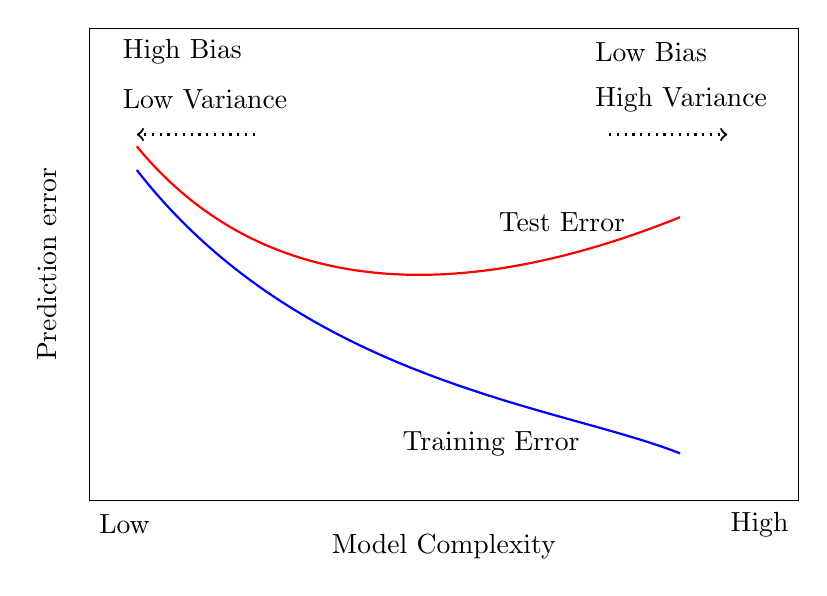
\begin{tikzpicture}[scale=3]
        \draw[] (0,0) rectangle (3,2);
        \draw[red, thick] (0.2,1.5) .. controls (0.9,0.65) and (2,1) .. (2.5,1.2);
        \draw[blue, thick] (0.2,1.4) .. controls (0.9,0.5) and (2,0.4) .. (2.5,0.2);
        \draw[->, dotted, thick] (0.7,1.55)--(0.2,1.55);
        \draw[->, dotted, thick] (2.2,1.55)--(2.7,1.55);
        \node[anchor=south] at (2,1.1) {Test Error};
        \node[anchor=south] at (1.7,0.15) {Training Error};
        \node[anchor=west] at (2.1,1.9) {Low Bias};
        \node[anchor=west] at (2.1,1.7) {High Variance};
        \node[anchor=west] at (0.1,1.9) {High Bias};
        \node[anchor=west] at (0.1,1.7) {Low Variance};
        \node[anchor=west] at (0,-0.1) {Low};
        \node[anchor=east] at (3,-0.1) {High};
        \node[anchor=south, rotate= 90] at (-0.1,1) {Prediction error};
        \node[anchor=north] at (1.5,-0.1) {Model Complexity};
    \end{tikzpicture}
    \fi
    \caption[Model complexity vs prediction error]{Illustration of how an increase in model complexity does not necessarily mean a lower prediction error when tested on new data. Thus, this can also be seen as an illustration of the Bias-Variance trade-off in model selection.}
    \label{fig:model_complexity}
\end{figure}

In search for the optimal model with the right complexity, one can constrain the hypothesis space to some extent.\footnote{The full hypothesis space is the space of all models ${f:\mathbb{R}^M \to \mathbb{R}}$, where $M$ is the number of features in the feature vector} For the sake of example, one could assume a linear relationship between the attributes, i.e., assuming that a target $y$ can be modelled as linear combinations of the features with weights $\bsw$ \eqref{lin_relation} 
\begin{equation}\label{eq:lin_relation}
    f\qty(\xxx,\bsw)  =  \xxx^{\top} \bsw  +w_0 
\end{equation} 

and thereby constrain the hypothesis space to the space of linear models.
In the supervised learning regime illustrated in \figref{supervised_learning}, we try to model inputs $\xxx$ to given outputs $y$, 
\begin{align}\label{eq:supervised_modelling}
    y&=f\qty(\xxx,\bsw) + \varepsilon
\end{align}
Where the modelling function $f\qty(\xxx,\bsw)$ is a function of the fixed feature vector $\xxx$ where the weights of the individual attributes are given as $\bsw$. The $\varepsilon$ parameter represents an unknown error term due to noise. The learning part of these supervised methods is then to optimize the weights based on the data set $\mathcal{D}$ in order to predict new observations accurately. Due to the results of this project being produced by a linear regression model, further elaboration of the linear regression model is considered appropriate.

\subsubsection{The Linear Regression Model}
The linear model assumes the targets $\yyy$ can be modelled as a linear function of the feature vector $\xxx$. Assuming that the data has been standardized (centered), the linear model are given as 
\begin{equation}\label{eq:lin_standard}
    f\qty(\xxx,\bsw) = \xxx^{\top} \bsw
\end{equation}

When trying to fit a proper model according to the machine learning method described in \secref{mlmethod}, one will then attempt to optimize the weights by minimizing a dissimilarity measure. The dissimilarity measure/error function used for the linear regression model is the residual sum of squares\index{Residual Sum of Squares} and the optimization \index{Optimization}problem is given as, 
\begin{equation}
    \bsw^* = \argmin_{\bsw} \curlyb{E\qty(\bsw)} = \argmin_{\bsw} \curlyb{\sum_{i=1}^{N} \qty(\hat{y}_i-\xxx^{\top} \bsw)^2}
\end{equation}
and with analysis, $\bsw^*$ can be found in terms of the data matrix $\XXX$ and the targets $\yyy$ as
\begin{equation}\label{eq:non_penalized_lin_model}
    \bsw^* = \qty( \XXXtilde^{\top} \XXXtilde )^{-1} \XXXtilde^{\top} \yyy
\end{equation}
Derivations of these results can be found in \appref{derivations}. 

\subsection{Penalization of the linear regression model}\label{sec:linmodel}
\index{Ordinary Least Squares}\index{Residual Sum of Squares}\index{Penalization}
As earlier stated, the linear regression model assumes that the targets can be predicted by linear combinations of the attributes of $\xxx$, which takes the form of \eqref{lin_relation}.   
The \emph{Ordinary Least Squares} (OLS) method is a linear regression model utilizing that the optimization of the weights is done using the \emph{residual sum of squares} (RSS) as the error function. The optimal weights $\bsw^*$ is then obtained by minimizing the residual sum of squares with respect to the weight vector\footnote{Again assuming that the data is centered, so that the bias weight $w_0$ can be neglected.}, $\bsw$, \begin{equation}\label{eq:ordinary_least_squares}
    \begin{split}
    \bsw^{*} = \argmin_{\bsw} \left\{\mathrm{RSS}\qty(\bsw) \right\} &= \argmin_{\bsw} \left\{ \sum_{i=1}^{N} \qty(\hat{y}_i - f\qty(\xxx_i))^2 \right\}\\
    &=\argmin_{\bsw} \left\{ \sum_{i=1}^{N} \qty( \hat{y}_i - \xxx^{\top} \bsw)^2 \right\}
    \end{split}
\end{equation}
A nice property of the linear regression is that it can be arbitrarily complex and take non-linear relations into account by introducing feature transformations, described in \secref{dataprep}, i.e., one can account for non-linear relationships by introducing feature transformations such as squaring the initial attributes. These feature transformations can exploit other proportionalities between the feature vectors and targets, but they increase the model complexity \index{Model Complexity} as well, which might result in overfitting the data. Thus, the optimization problem can be restated as finding the perfect balance between bias and variance, as illustrated in \figref{model_complexity}. The \emph{bias-variance trade-off} can be taken into consideration by penalizing the error function. Examples of such penalizations are the Lasso and the Ridge regressions. The benefits of applying coefficient shrinkage like Lasso\index{Lasso} and Ridge \index{Ridge Regression}is not just the consideration of the bias-variance trade-off\index{Bias-Variance Trade-off}, but both regression\index{Regression} types also increase the interpretability of a given model due to the fact that they allow weights for irrelevant attributes to shrink towards zero.

\subsubsection{Least Absolute Shrinkage and Selection Operator (Lasso)}
Like OLS, Lasso optimizes the residual sum of squares with respect to the weights, but adds the constraint that the sum of absolute values of weights should be less or equal to some shrinkage parameter $s$ which has to be chosen appropriately. Thus the formal formulation for the Lasso method is as \eqref{ordinary_least_squares} under the extra constraint that,
\begin{equation}\label{eq:lasso_shrinkage_constraint}
\sum_{j=1}^{M} \left| w_j \right| \leq s
\end{equation}
If the $s$ parameter is less than the full OLS estimate, this penalization will cause the weights of less important attributes to shrink until some truncate at $w_k=0$ is reached in order to fulfill \eqref{lasso_shrinkage_constraint}. This is equivalent to the problem of minimizing: 
\begin{equation}\label{eq:lasso_prob}
    \bsw^{*} = \argmin_{\bsw} \left\{ \sum_{i=1}^{N} \qty(y_i -\bsw^{\top} \xxx_i)^2 + \lambda \sum_{j=1}^{M} \left| w_j \right| \right\}
\end{equation}
where the value of $\lambda$ indicates the amount of shrinkage, i.e., a bigger value of $\lambda$ implies more shrinkage and thus more bias added to the model and vice versa with smaller values of $\lambda$ which means that less bias is introduced.\footnote{$\lambda$ is generally referred to as the regularization strength and usually takes on values in the range of $10^{-5}$ to 1.} Regularization is thus a method of substantially reducing the variance of a model without introducing too much bias if $\lambda$ is chosen wisely. The concepts of regularization arises naturally from probability theory by acknowledging that the prior probability distribution of the weights, $p\qty(\bsw)$ is not supposed to be ignored/assumed uniform in the derivation of the OLS.\footnote{However, proof of this statement will not be included in this project, but can be found in a lot of literature, e.g. \citep{allhailkingMorten}}


\paragraph{The difference between Lasso and Ridge} lies in the \Lnorm{p} used to penalize the residual sum of squares. Whereas Lasso uses the \Lnorm{1}, Ridge regression regularizes using a \Lnorm{2}.\footnote{This results in the solutions to the optimization problem for Lasso being non-linear in $y$ while the solutions to the Ridge optimization problem is linear in $y$} To understand the difference between the two penalization types, the geometry of Lasso and Ridge will be studied briefly using the OLS criterion which is equivalent to the quadratic function,
\begin{align}
    \qty(\bsw - \bsw^0)^{\top} \XXXtilde^{\top} \XXXtilde (\bsw - \bsw^0)+C
\end{align}
where $\bsw^0$ is the full OLS estimate without shrinkage and $C$ is a constant. In \figref{lassovsridge}, the contours of this quadratic function are outlined as well as the constraint regions for the Lasso ($L_1$-norm) and Ridge ($L_2$-norm) respectively. In the two dimensional case of \figref{lassovsridge} it is seen that the contours can hit the tip of the constraint region in the Lasso case. If this happens, one of the two weights will become equal to zero. In the Ridge case, the weights can only become $\approx 0$. This two dimensional example can easily be expanded and hence the Lasso allows for sparse solutions in regards to the number of features. 

The decision about whether to apply a Lasso- or Ridge penalization, as usual, requires the machine learning practitioner to think about the data set in hand. According to the results found by \citep{Tibshirani94regressionshrinkage}, the Ridge penalization is performing better than Lasso when the target values can be predicted by many small effects, whereas Lasso performs best when there is a small to moderate number of features that contribute to predict the targets, as \figref{lassovsridge} suggests as well.

In this project, we would like to create an as low dimensional feature vector as possible, i.e. look for the smallest set of features being able to predict the targets of our model fairly accurately. Hence, the \Lnorm{1} seems like the preferable choice of regularization. However, since we would like to find the smallest possible set of features able to predict our targets, it is worth considering sequential feature selection.\index{Sequential Feature Selection}\index{Forward Selection}

\paragraph{Forward selection} iterates through the features one by one and adds the feature with the lowest test error $E_{\mathrm{test}}$ to the optimal set of features. It then tries to add another feature to the feature vector by searching for candidates that can lower the error compared to the single feature. If multiple features can lower $E_{\mathrm{test}}$, the one that results in the largest decrease in test error will be chosen. The algorithm then continues until the test error cannot be decreased by addition of another feature. According to \citep{Tibshirani94regressionshrinkage}, this method is preferable when there is a small amount of large effects, i.e. a small amount of highly important features.
%%%%%%%%%%%%%%%%%%%%%%%%%%%%%%%%%%%
%   Lasso vs Ridge penalty plot   %
%%%%%%%%%%%%%%%%%%%%%%%%%%%%%%%%%%%

\begin{figure}[t]
    \centering
    %First pictures
   
    \begin{subfigure}[b]{0.45\textwidth}
    \iffigure
        \begin{tikzpicture}
            \begin{axis}[no markers,xlabel=$\hat{w}_1$, 
                ylabel=$\hat{w}_2$,
                ticks=none,
                axis x line=center,
                axis y line=center,
                ymin=-1.1,
                xmin=-1.1,
                xmax=2,
                ymax=3,
                axis equal]
                \addplot+[fill=softblue, color=softblue, opacity=0.5] coordinates
                {(-1,0) (0,1) (1,0) (0,-1)}--cycle;
                \draw[red] (1,2) ellipse [x radius=0.4, y radius=0.2, rotate=45];
                \draw[red] (1,2) ellipse [x radius=0.6, y radius=0.3, rotate=45];
                \draw[red] (1,2) ellipse [x radius=1, y radius=0.5, rotate=45];
                \draw[red] (1,2) ellipse [x radius=1.4, y radius=0.7, rotate=45];
                \node[] at (1,2) {$\hat{w}$};
            \end{axis}
            %
        \end{tikzpicture}
        \fi
    \end{subfigure}
    \quad
    %Second picture
    \begin{subfigure}[b]{0.45\textwidth}
    \iffigure
        \begin{tikzpicture}
            \begin{axis}[no markers,xlabel=$\hat{w}_1$, 
                ylabel=$\hat{w}_2$,
                ticks=none,
                axis x line=center,
                axis y line=center,
                ymin=-1.1,
                xmin=-1.1,
                xmax=2,
                ymax=3,
                axis equal]
                \filldraw[draw=softblue, fill=softblue, opacity=0.5] (0,0) circle (1);
                \draw[red] (1,2) ellipse [x radius=0.4, y radius=0.2, rotate=45];
                \draw[red] (1,2) ellipse [x radius=0.6, y radius=0.3, rotate=45];
                \draw[red] (1,2) ellipse [x radius=1, y radius=0.5, rotate=45];
                \draw[red] (1,2) ellipse [x radius=1.3, y radius=0.65, rotate=45];
                \node[] at (1,2) {$\hat{w}$};
            \end{axis}
        \end{tikzpicture}
        \fi
    \end{subfigure}
    
    \caption[Lasso versus Ridge Shrinkage]{Illustration of how the Least Absolute Shrinkage and Selection Operator (Lasso) is able to set some weights of features to 0 (using the \Lnorm{1}) whereas Ridge regression only allow specific feature weights to be $\approx$ 0 but $\neq$ 0 (using the \Lnorm{2}). The figure on the left shows a \Lnorm{1} and on the right a \Lnorm{2}.}
    \label{fig:lassovsridge}
\end{figure}

%%%%%%%%%%%%%%%%%%%%%%%%%%%%%%%%%%%%

\seclab{Model selection and performance Evaluation}{mspe}\index{Model Selection}\index{Performance Evaluation}
When performing model selection, one should assess the optimal model as the model which generalizes best to unseen data, i.e., to search for the model that will minimize the test error curve in \figref{model_complexity}. But the test error is specific to a given test, hence, to get the true prediction error, one would like to test the model on as much unseen data as possible and ideally, an infinite amount of data. The generalization error, which is an idealized quantity, is introduced as the error the model would have, had it been tested on an infinite amount of test data $\notin$ $\mathcal{D}_{\mathrm{train}}$.

\subsection{Cross-validation}\label{sec:crossvalidation}\index{Cross-Validation}

\begin{figure}[ht]
    \centering
    \iffigure
    \begin{tikzpicture}
    
        %First line
        \filldraw[draw=softblue, fill=softblue] (0,3.5) rectangle (12,4.5);
        % third line
        \filldraw[draw=softblue, fill=softblue] (0,2) rectangle (12,3);
        \filldraw[draw=softgrey, fill=softgrey] (0,2) rectangle (4,3);
        %fourth line
        \filldraw[draw=softblue, fill=softblue] (0,0.5) rectangle (12,1.5);
        \filldraw[draw=softgrey, fill=softgrey] (4,0.5) rectangle (8,1.5);
        %fith line
        \filldraw[draw=softblue, fill=softblue] (0,-1) rectangle (12,0);
        \filldraw[draw=softgrey, fill=softgrey] (8,-1) rectangle (12,0);
        %Legend
        \node[] at (6,4) {$N$};
        
        \node[] at (2,2.5) {$\dfrac{1}{3}N$ };
        \node[] at (8,2.5) {$\dfrac{2}{3}N$ };
        
        \filldraw[draw=softblue, fill=softblue] (0,5) rectangle (0.5,5.5);
        \node[anchor=west] at (0.5,5.25) {Training data};
        
        \filldraw[draw=softgrey, fill=softgrey] (9.5,5) rectangle (10,5.5);
        \node[anchor=west] at (10,5.25) {Test data};
        
        
    \end{tikzpicture}
    \fi
    \caption[Cross-validation illustration]{Visual example of $K$-fold CV; Here seen a 3-fold validation where the data set is split into subsets, $\mathcal{D} = \mathcal{D}_1 \cup \mathcal{D}_2 \cup \mathcal{D}_3 $. For each subset, the model is trained on 2/3 and tested on 1/3 of the total $N$ observations.}
    \label{fig:kfold}
\end{figure}


\emph{Cross-validation} (CV) is a technique which beautifully takes into account, that when finding the optimal model for a problem, one must not test the model on the data used for training. The idea behind CV, is to create as much test and training data using only the data set itself. There are three major types of cross-validation, \emph{Hold-Out} CV, \emph{K}-fold CV and \emph{Leave-one-out} Cross-validation\citep{allhailkingMorten}. In this project, \emph{K}-fold has been used exclusively. Both for model selection and estimating the generalization error of the optimal model. When performing $K$-fold CV, the data set is split into $K$ subsets, $\mathcal{D} = \mathcal{D}_1 \cup  ... \cup \mathcal{D}_k \cup ... \cup \mathcal{D}_K$. Hence, $K$-fold CV allows one to test the models on the entire data set.

In $K$-fold CV, the idealized generalization error \index{Generalization Error} is approximated as:
\begin{equation}\label{eq:gen_error}
    \EM{gen} \approx \sum_{k=1}^K \dfrac{N_{k}^{\mathrm{test}}}{N}   E_{\mathcal{M},k}^{\mathrm{test}}
\end{equation}
where $N_k^{\mathrm{test}}$ is the number of observations for testing in fold number $k$, and $\EMss{,k}{test}$ is given as
\begin{equation}
    \EMss{,k}{test} = \dfrac{1}{N_{k}^{\mathrm{test}}} \sum_{i \in \Dtest} d\qty(y_i,\FM{\xxx_i,\bsw})
\end{equation}
The appropriate dissimilarity measure varies from task to task, but recall that in the case of regression, one uses the RSS. An illustrative example of how the data is split for a $3$-fold CV is seen in \figref{kfold}.

CV can be used for both model selection and estimation of the generalization error. Two-layer CV is a way of doing both and thus getting an unbiased estimate of the generalization error. This is done for every model created in the code phase of this project. Therefore the procedure is outlined in pseudo-code in Algorithm \ref{algo:tlcv}\footnote{The idea of outlining the Algorithm in pseudo-code is due to \citep{allhailkingMorten}}.
\begin{algorithm}
\caption{$K$-Fold Cross-Validation for Model selection and $\EM{gen}$ estimation}

\begin{algorithmic}[0]

\Require{$K_1$ folds in outer loop for estimation of the generalization error}
\Require{$K_2$ folds in inner loop for model selection}
\Require{$S$ models to cross-validate: $\mathcal{M}_1 , ... , \mathcal{M}_S$}
\Ensure{$\hat{E}_{\mathcal{M}*}^{\mathrm{gen}}$}

\For{$i =1,...,K_1$}
    \State{\emph{Outer CV loop. The data set, $\calD$ is split into $K_1$ folds} }
    \State{The $i$'th split of $\calD$ is $\calD_{i}^{\mathrm{par}},\calD_{i}^{\mathrm{test}}$}
    \For{$j=1,...,K_2$}
        \State{\emph{Inner CV loop doing $K_2$ splits for model selection testing $S$ models}}
        \State{The $j$'th split of $\calD_i^{\mathrm{par}}$ is $\calDss{j}{train},\calDss{j}{val}$} 
        \For{$s=1,...,S$}
            \State{Train $\mathcal{M}_s$ on $\calDss{j}{train}$ }
            \State{Let $\EMss{_{s,j}}{val}$ be the \emph{validation error} of the model $\mathcal{M}_s$ when it is \emph{tested} on $\calDss{j}{val}$}
        \EndFor
    \EndFor    
    \State{For each $s$ compute $\hat{E}_s^{\mathrm{gen}}= \sum_{j=1}^{K_2} \frac{\abs{\calDss{j}{val}}}{\calDss{i}{par}} \EMss{_s,j}{val}$ }
    \State{Select the optimal model $\mathcal{M}^*$ = $\mathcal{M}_{s^*}$ where $s^* = \argmin_s \hat{E}_s^{\mathrm{gen}}$}
    \State{Train $\mathcal{M}^*$ on $\calDss{i}{par}$}
    \State{Let $E_i^{\mathrm{test}}$ be the \emph{test error} of the model $\mathcal{M}^*$ when it is tested on $\calDss{i}{test}$}
\EndFor
\State{Compute the estimate of the generalization error: $\hat{E}^{\mathrm{gen}} = \sum_{i}^{K_1} \frac{\abs{\calDss{i}{test}}}{N} E_i^{\mathrm{test}}$}
\end{algorithmic}
\label{algo:tlcv}
\end{algorithm}







